% ============================================================================
%  Section 3: Data and Estimation
%  Sources: FROT 2025_sub/5_quantitative_model.tex (Estimation, Match of Moments),
%           FROT 2025_sub/11_app_data.tex (data appendix), FROT 2025_sub/12_app_quant.tex (MSM),
%           FROT v6/12_app_quant_resubmission_v6.tex (fit wording, lines 108--242).
% ============================================================================
\section{Data and Estimation}\label{sec:estimation}

We estimate the model of Section~\ref{sec:model} on US panel data for the cohorts born between 1920 and 1940 and show that the estimated economy reproduces the life-cycle profiles of participation, hours, and wealth by health status on which the reform analysis rests.

\subsection{Estimation Strategy}

We follow the two-step strategy that is standard for structural life-cycle models \citep{Gourinchas2002,Cagetti2003}. In the first step, we estimate or calibrate the parameters that can be identified without solving the model: the age profiles of health transitions, survival, out-of-pocket medical expenses, and wages by health status, together with the stochastic process for ability, all estimated directly from the data; the interest rate and the consumption floor, taken from the literature; and the parameters of Social Security, disability insurance, pensions, and taxes, taken from program rules and earlier work. We collect these first-step parameters in a vector $\chi$. In the second step, we estimate the preference parameters
\[
\mathcal{P}=\big(\gamma,\ \nu,\ \beta,\ L,\ \phi_n(0),\ \phi_n(1)=\phi_n(2),\ \phi_{RE}\big)
\]
by the method of simulated moments (MSM), taking $\chi$ as given: we search for the parameter vector whose simulated life-cycle profiles are closest to their counterparts in the data.

The division between the two steps mirrors what a retirement reform changes. The first-step objects---how health evolves, how it shifts wages, mortality, and medical spending, and what the programs pay---are constraints that the reforms of Section~\ref{sec:results} leave unchanged, except for the program rules each reform alters. The second-step parameters govern how individuals respond when those rules change. The fixed costs of participation determine how many workers are close to the margin between working and retiring; the reentry cost determines whether a retirement decision can be undone; and the curvature parameters $\gamma$ and $\nu$, together with the discount factor $\beta$, determine the value of insurance and the strength of income effects. Because both the willingness to pay and the fiscal externalities of Section~\ref{sec:framework} are functions of these responses, we discipline the second step with the profiles that reflect them most directly: participation and hours by health status, wealth, and labor market reentry.

The estimation builds on \citet{french2005effects} and \citet{french2011effects} and departs from them in two respects. First, the target profiles describe the whole population of the cohorts---household heads and their spouses---rather than male household heads, so that the aggregate fiscal accounts used to compute MVPFs refer to the population the reforms reach. Second, the fixed cost of participation depends on health. It is identified from the gap between the participation profiles of healthy and unhealthy individuals that remains once the first step has accounted for the differences in wages, mortality, medical expenses, and access to disability insurance across health states.

\subsection{Data}

\paragraph{Panel Study of Income Dynamics.} Our main data source is the Panel Study of Income Dynamics (PSID), a longitudinal survey of a representative sample of the US population that records labor market outcomes, income, health, and wealth. The PSID began in 1968 with interviews of about 4,800 families % Source: FROT 2025_sub/11_app_data.tex
and has followed these families and their descendants annually until 1997 and biennially since. We use the 1968--2015 waves. We restrict the sample to the nationally representative Survey Research Center component, excluding the low-income Survey of Economic Opportunity subsample, most of which was dropped from the survey after 1997, and keep household heads and spouses aged 20 to 90 with nonmissing labor and health information. % Source: FROT 2025_sub/11_app_data.tex, tables/sample_psid.tex

We focus on individuals born between 1920 and 1940 for two reasons. First, these cohorts were subject to similar Social Security rules: an early retirement age (ERA) of 62, on average a normal retirement age (NRA) of 65, and a delayed retirement credit (DRC) that rose with the year of birth and whose cohort average, 4.5 percent, we use in the model. A single policy environment therefore describes the incentives behind the retirement behavior we observe. Second, the PSID observes these cohorts over most of the life cycle: the youngest cohort is 28 years old in the first wave, and the oldest cohorts are observed well past the ages at which retirement decisions are made. The final sample contains 2,248 individuals and 44,404 person--year observations (\autoref{tab:sample_psid}). % Source: FROT 2025_sub/11_app_data.tex

\paragraph{Medical Expenditure Panel Survey.} We measure medical spending in the Medical Expenditure Panel Survey (MEPS), a nationally representative survey of families and individuals, their medical providers, and employers, with detailed information on medical expenditures, sources of payment, insurance coverage, and health status. Spending is reported at the individual level and cross-checked with providers and insurers. We use the 1999--2012 waves, keep household heads aged 20 and older, and drop observations with missing age, medical spending, insurance coverage during working ages, or health status, which leaves 120,731 individuals and 211,709 person--year observations (\autoref{tab:sample_meps}). % Source: FROT 2025_sub/11_app_data.tex, tables/sample_meps.tex

\paragraph{Health.} Health enters every first-step profile, so it must be measured consistently over the entire life cycle. In the PSID, we use three self-reported work-limitation questions asked in every wave and classify individuals, following \citet{Low2015}, as in good health ($h=0$) if they report no work-limiting condition or a condition that does not limit the amount of work; in poor health ($h=1$) if a condition limits the amount of work somewhat or a little; and as having a disability ($h=2$) if the condition prevents them from doing any work and limits the amount of work a lot, which corresponds to the Social Security Administration (SSA) criterion for disability insurance (DI). Alternative measures, such as the frailty index of \citet{Hosseini2021} and self-rated health, are available in the PSID only for later waves and cannot describe the health dynamics of these cohorts over their life cycle. In the MEPS, we follow \citet{Pashchenko2019} and use self-rated health on a five-point scale: an individual is in good health if she reports excellent, very good, or good health in all three interviews of a year, has a disability if she reports poor health in any interview, and is in poor health otherwise. The two classifications agree closely on the share of people with a disability and on the decline of good health with age (\autoref{tab:health_measures}), which allows us to combine transition, survival, and wage profiles from the PSID with medical-expense profiles from the MEPS. Appendix~\ref{app:data} reports the survey questions and the sample construction.

\paragraph{Target profiles.} The second step targets four PSID profiles over ages 30 to 69. Labor force participation equals one if annual hours exceed 800, which counts both full-time and part-time work; % Source: FROT 2025_sub/11_app_data.tex (Target Profiles)
hours are annual hours of participants; assets are nonpension net worth, which excludes pension and Social Security wealth; and reentry is participation after a year out of the labor force. Participation and hours are measured separately for healthy individuals ($h=0$) and unhealthy individuals ($h\in\{1,2\}$), which we pool because the PSID contains few observations of people with a disability at each age; assets and reentry are not conditioned on health. We purge the profiles of family-size, business-cycle, and individual fixed effects with the procedure of \citet{french2005effects}, described in Appendix~\ref{app:msm}. Monetary values are in 2016 dollars.

\subsection{First-Step Estimates}

\paragraph{Health, survival, and medical expenses.} For each health state $i$, we estimate the transition probabilities $\pi_{j,i,t+1}$ from probit regressions of an indicator for next-period health $j$ on a full set of age dummies, using the observations in state $i$, and interpolate the predicted probabilities linearly across ages. Survival probabilities $S(h,t)$ come from a logistic regression of survival on a polynomial in age, lagged health, and their interactions (\autoref{tab:survival}). Out-of-pocket medical expenses $M(\cdot)$ are total medical expenditures in the MEPS net of the share covered by insurance before age 65 and by Medicare from age 65, estimated by age and health status and scaled to the aggregates of the National Health Expenditure Accounts following \citet{Denardi2018}.

Panels A to C of \autoref{fig:firststep} display the resulting profiles. The probability of remaining in good health falls steadily with age, and the decline is absorbed mostly by transitions into poor health (panel A). Mortality rises with age in every health state, and much faster for people with a disability (panel B). Out-of-pocket medical expenses rise with age and are considerably higher in poor health and with a disability (panel C). Each profile gives health an independent role in retirement: worse health shortens the expected horizon over which a delayed claim pays off and raises the medical risk against which retirees self-insure.

\paragraph{Wages.} Hourly wages are annual earnings divided by annual hours in the PSID. Because wages are observed only for participants, and those who keep working when old or unhealthy are likely to be those with high offered wages, observed wages would overstate offered wages precisely for the groups whose retirement decisions matter most. We correct for this selection with the two-step estimator of \citet{Heckman1976}, as in \citet{Guner2012}. A participation probit on all PSID observations generates an inverse Mills ratio, which enters a regression of log wages on an age polynomial and its interactions with health. Family size and year of birth enter the selection equation but not the wage equation (\autoref{tab:wages}). The coefficient on the inverse Mills ratio is positive and significant, so participants are positively selected and the correction lowers the offered-wage profiles of groups with low participation. \citet{french2005effects} and \citet{french2011effects} instead correct for selection inside the structural estimation; estimating the wage profiles outside the model keeps them invariant to the preference parameters and reduces the computational burden of the second step. Healthy individuals earn higher hourly wages than individuals in poor health, who in turn earn more than individuals with a disability, at every age (panel D of \autoref{fig:firststep}).

We estimate the ability process \eqref{eq:ability} from the wage residuals by maximum likelihood with the Kalman filter. The process is highly persistent, with autoregressive coefficient and innovation variance $(\rho,\sigma^2)=(0.981,0.016)$. Wage shocks are therefore close to permanent: a worker hit by an adverse shock in her 50s expects lower wages throughout the retirement window, which brings forward the date at which the value of leisure overtakes the value of work.

\paragraph{Calibrated parameters and program rules.} We set the gross interest rate to $r_f=4$ percent, as in \citet{french2005effects}, and the wedge between the gross and the net return to 20 percent, as in \citet{Stantcheva2017}, which captures corporate and other direct capital taxes not represented in the income tax function; the net return is $r=3.2$ percent. The consumption floor is $\underline{c}=\$3{,}500$ \citep{french2011effects}. The age-dependent income tax function is estimated from the PSID as in \citet{Borella2023}. Social Security rules are those that applied to the 1920--1940 cohorts (\autoref{tab:ssparams}); disability benefits are scaled by the probability of a successful DI application estimated by \citet{Low2015}; and pension benefits follow \citet{french2005effects}, with parameters from \citet{Gustman1999} and age-specific accruals from \citet{Gustman2000}. The initial joint distribution of assets, wages, health, and participation at age 30 is drawn from the PSID (\autoref{tab:initial}). \autoref{tab:calibrated} summarizes the first-step inputs, and Appendix~\ref{app:firststep} details each estimation.

\begin{figure}[!htbp]
\centering
\caption{First-Step Estimates: Profiles by Health Status}\label{fig:firststep}
\vspace{0.5em}
% Panels copied verbatim from the FROT project (figures/abdou/*.tex), arranged as in FROT 2025_sub/5_quantitative_model.tex.
\begin{tabular}{@{}c@{\hspace{1.5em}}c@{}}
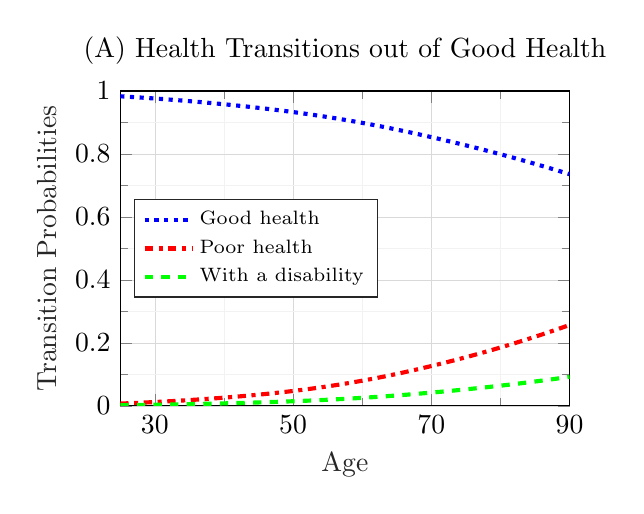
\begin{tikzpicture}
\begin{axis}[%
width=5.706cm,
height=4cm,
at={(0cm,0cm)},
scale only axis,
xmin=25,
xmax=90,
xtick={30,50,70,90},
xlabel style={font=\color{white!15!black}},
xlabel={Age},
ymin=0,
ymax=1,
ylabel style={font=\color{white!15!black}},
ylabel={Transition Probabilities},
axis background/.style={fill=white},
%title style={font=\bfseries},
title={(A) Health Transitions out of Good Health},
legend style={at={(0.03,0.5)}, anchor=west, legend cell align=left, align=left, draw=white!15!black,font=\scriptsize},
grid=both,
grid style={line width=0.2pt, draw=gray!30},
minor grid style={line width=0.1pt, draw=gray!10},
minor tick num=1
]
% Blue line - h(t)=0 - dotted line
\addplot [color=blue, line width=1.5pt, dotted]
  table[row sep=crcr]{%
25 0.98309247\\
26 0.98177065\\
27 0.98040043\\
28 0.97898087\\
29 0.97751107\\
30 0.97599011\\
31 0.97441706\\
32 0.97279099\\
33 0.97111097\\
34 0.96937609\\
35 0.96758542\\
36 0.96573805\\
37 0.96383308\\
38 0.96186959\\
39 0.95984659\\
40 0.95776298\\
41 0.95561743\\
42 0.95340817\\
43 0.95113281\\
44 0.94878801\\
45 0.94636924\\
46 0.94387079\\
47 0.94128627\\
48 0.93861018\\
49 0.93583981\\
50 0.93297328\\
51 0.93000876\\
52 0.92694444\\
53 0.92377856\\
54 0.92050939\\
55 0.91713528\\
56 0.91365461\\
57 0.91006583\\
58 0.90636744\\
59 0.90255801\\
60 0.89863619\\
61 0.89460071\\
62 0.89045035\\
63 0.88618399\\
64 0.88180192\\
65 0.87730914\\
66 0.87271271\\
67 0.86801917\\
68 0.86323358\\
69 0.85835934\\
70 0.85339844\\
71 0.84835184\\
72 0.8432198\\
73 0.83800218\\
74 0.83269856\\
75 0.82730842\\
76 0.82183118\\
77 0.81626625\\
78 0.81061306\\
79 0.80487101\\
80 0.79903956\\
81 0.79311816\\
82 0.78710628\\
83 0.78100339\\
84 0.77480897\\
85 0.76852255\\
86 0.76214369\\
87 0.75567204\\
88 0.74910741\\
89 0.74244985\\
90 0.73569986\\
};
\addlegendentry{Good health}

% Red line - h(t)=1 - dash-dotted line
\addplot [color=red, line width=1.5pt, dashdotted]
  table[row sep=crcr]{%
25 0.00740989\\
26 0.00829385\\
27 0.0092242\\
28 0.01020239\\
29 0.01122993\\
30 0.01230832\\
31 0.01343908\\
32 0.01462377\\
33 0.01586393\\
34 0.01716114\\
35 0.01851696\\
36 0.01993295\\
37 0.02141069\\
38 0.02295175\\
39 0.02455777\\
40 0.02623054\\
41 0.02797205\\
42 0.02978474\\
43 0.03167175\\
44 0.0336372\\
45 0.03568655\\
46 0.03782661\\
47 0.04006511\\
48 0.04240901\\
49 0.04486246\\
50 0.04742877\\
51 0.05011122\\
52 0.05291311\\
53 0.05583768\\
54 0.05888815\\
55 0.0620677\\
56 0.06537945\\
57 0.06882647\\
58 0.07241176\\
59 0.07613823\\
60 0.08000872\\
61 0.08402595\\
62 0.08819256\\
63 0.09251107\\
64 0.09698204\\
65 0.10159943\\
66 0.10635428\\
67 0.1112381\\
68 0.11624445\\
69 0.12136908\\
70 0.1266097\\
71 0.13196542\\
72 0.13743634\\
73 0.14302316\\
74 0.14872693\\
75 0.15454888\\
76 0.16049033\\
77 0.16655263\\
78 0.1727371\\
79 0.17904508\\
80 0.18547785\\
81 0.1920367\\
82 0.19872287\\
83 0.20553761\\
84 0.21248211\\
85 0.21955753\\
86 0.22676493\\
87 0.23410525\\
88 0.24157916\\
89 0.24918697\\
90 0.25692832\\
};
\addlegendentry{Poor health}

% Green line - h(t)=2 - dashed line
\addplot [color=green, line width=1.5pt, dashed]
  table[row sep=crcr]{%
25 0.00232342\\
26 0.00258882\\
27 0.00286849\\
28 0.00316296\\
29 0.00347276\\
30 0.00379847\\
31 0.00414063\\
32 0.00449986\\
33 0.00487673\\
34 0.00527188\\
35 0.00568592\\
36 0.00611948\\
37 0.00657321\\
38 0.00704778\\
39 0.00754387\\
40 0.00806223\\
41 0.0086037\\
42 0.00916924\\
43 0.00976009\\
44 0.0103778\\
45 0.01102439\\
46 0.01170237\\
47 0.0124146\\
48 0.01316373\\
49 0.01395159\\
50 0.01477974\\
51 0.0156498\\
52 0.01656341\\
53 0.01752226\\
54 0.01852807\\
55 0.01958259\\
56 0.02068762\\
57 0.02184496\\
58 0.02305648\\
59 0.02432406\\
60 0.02564961\\
61 0.02703505\\
62 0.02848236\\
63 0.02999351\\
64 0.03156963\\
65 0.03320868\\
66 0.03490704\\
67 0.03666119\\
68 0.03846841\\
69 0.040327\\
70 0.04223612\\
71 0.04419564\\
72 0.04620591\\
73 0.04826763\\
74 0.05038168\\
75 0.05254912\\
76 0.05477106\\
77 0.0570487\\
78 0.05938328\\
79 0.06177607\\
80 0.0642284\\
81 0.06674166\\
82 0.06931726\\
83 0.07195667\\
84 0.07466143\\
85 0.07743309\\
86 0.08027324\\
87 0.08318347\\
88 0.08616529\\
89 0.08922008\\
90 0.0923489\\
};
\addlegendentry{With a disability}
\end{axis}
\end{tikzpicture} & 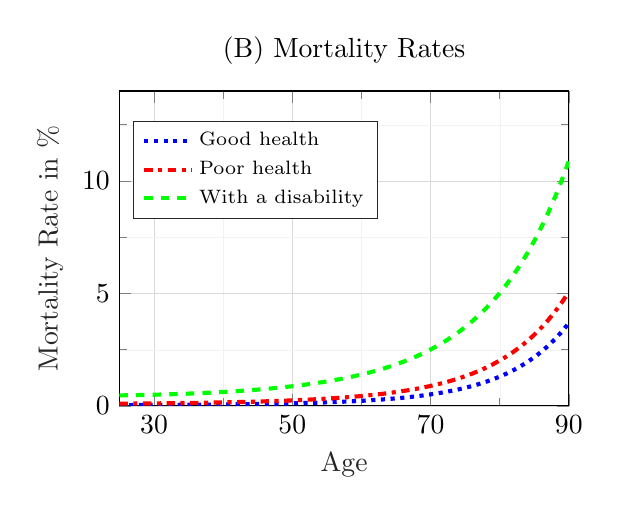
\begin{tikzpicture}
\begin{axis}[%
width=5.706cm,
height=4cm,
at={(0cm,0cm)},
scale only axis,
xmin=25,
xmax=90,
xtick={30,50,70,90},
xlabel style={font=\color{white!15!black}},
xlabel={Age},
ymin=0,
ymax=14,
ylabel style={font=\color{white!15!black}},
ylabel={Mortality Rate in \%},
axis background/.style={fill=white},
%title style={font=\bfseries},
title={(B) Mortality Rates},
legend style={at={(axis cs:27,10.5)}, anchor=west, legend cell align=left, align=left, draw=white!15!black, font=\scriptsize},
grid=both,
grid style={line width=0.2pt, draw=gray!30},
minor grid style={line width=0.1pt, draw=gray!10},
minor tick num=1
]
% Back line (Overall) - full
% \addplot [color=black, line width=1.5pt]
%   table[row sep=crcr]{%
% 25 0.04479\\
% 26 0.04675\\
% 27 0.0481\\
% 28 0.05082\\
% 29 0.05277\\
% 30 0.05375\\
% 31 0.05639\\
% 32 0.05905\\
% 33 0.06249\\
% 34 0.06579\\
% 35 0.06926\\
% 36 0.07637\\
% 37 0.07822\\
% 38 0.08325\\
% 39 0.08796\\
% 40 0.09379\\
% 41 0.09919\\
% 42 0.10925\\
% 43 0.11504\\
% 44 0.12074\\
% 45 0.12909\\
% 46 0.13868\\
% 47 0.1475\\
% 48 0.15626\\
% 49 0.16962\\
% 50 0.18554\\
% 51 0.20082\\
% 52 0.21588\\
% 53 0.23697\\
% 54 0.25106\\
% 55 0.27595\\
% 56 0.30314\\
% 57 0.32832\\
% 58 0.35589\\
% 59 0.38782\\
% 60 0.41329\\
% 61 0.45229\\
% 62 0.48501\\
% 63 0.52826\\
% 64 0.55276\\
% 65 0.59562\\
% 66 0.66072\\
% 67 0.70075\\
% 68 0.74535\\
% 69 0.80985\\
% 70 0.87603\\
% 71 1.00144\\
% 72 1.03708\\
% 73 1.21095\\
% 74 1.28609\\
% 75 1.47924\\
% 76 1.53636\\
% 77 1.74536\\
% 78 1.86332\\
% 79 2.00865\\
% 80 2.31624\\
% 81 2.51996\\
% 82 2.79552\\
% 83 3.17659\\
% 84 3.35743\\
% 85 3.97544\\
% 86 4.09512\\
% 87 4.87983\\
% 88 5.39166\\
% 89 6.00628\\
% 90 6.48326\\
% };
% \addlegendentry{Overall}
% Blue line (Good health) - dotted
\addplot [color=blue, line width=1.5pt, dotted]
  table[row sep=crcr]{%
25 0.035\\
26 0.03614\\
27 0.03736\\
28 0.03868\\
29 0.04009\\
30 0.0416\\
31 0.04323\\
32 0.04497\\
33 0.04685\\
34 0.04886\\
35 0.05103\\
36 0.05335\\
37 0.05586\\
38 0.05855\\
39 0.06146\\
40 0.06458\\
41 0.06795\\
42 0.07159\\
43 0.07552\\
44 0.07975\\
45 0.08434\\
46 0.0893\\
47 0.09467\\
48 0.10049\\
49 0.1068\\
50 0.11365\\
51 0.12109\\
52 0.12917\\
53 0.13798\\
54 0.14756\\
55 0.158\\
56 0.1694\\
57 0.18184\\
58 0.19545\\
59 0.21032\\
60 0.22662\\
61 0.24448\\
62 0.26407\\
63 0.28558\\
64 0.30923\\
65 0.33525\\
66 0.3639\\
67 0.39548\\
68 0.43033\\
69 0.46882\\
70 0.51137\\
71 0.55844\\
72 0.61059\\
73 0.66839\\
74 0.73254\\
75 0.80378\\
76 0.88297\\
77 0.97108\\
78 1.06919\\
79 1.17854\\
80 1.3005\\
81 1.43664\\
82 1.58871\\
83 1.75871\\
84 1.94885\\
85 2.16166\\
86 2.39997\\
87 2.66694\\
88 2.96613\\
89 3.30152\\
90 3.67755\\
};
\addlegendentry{Good health}

% Red line (Poor health) - dash-dotted
\addplot [color=red, line width=1.5pt, dashdotted]
  table[row sep=crcr]{%
25 0.09962\\
26 0.10175\\
27 0.10405\\
28 0.10654\\
29 0.10922\\
30 0.11212\\
31 0.11523\\
32 0.11858\\
33 0.12218\\
34 0.12605\\
35 0.1302\\
36 0.13466\\
37 0.13944\\
38 0.14458\\
39 0.15009\\
40 0.15601\\
41 0.16236\\
42 0.16919\\
43 0.17652\\
44 0.18441\\
45 0.19288\\
46 0.202\\
47 0.21181\\
48 0.22237\\
49 0.23376\\
50 0.24603\\
51 0.25927\\
52 0.27356\\
53 0.289\\
54 0.30569\\
55 0.32375\\
56 0.3433\\
57 0.36448\\
58 0.38745\\
59 0.41237\\
60 0.43943\\
61 0.46884\\
62 0.50084\\
63 0.53568\\
64 0.57364\\
65 0.61503\\
66 0.66022\\
67 0.70958\\
68 0.76354\\
69 0.82259\\
70 0.88726\\
71 0.95816\\
72 1.03592\\
73 1.12131\\
74 1.21513\\
75 1.31831\\
76 1.43187\\
77 1.55694\\
78 1.6948\\
79 1.84687\\
80 2.01472\\
81 2.20011\\
82 2.40499\\
83 2.63155\\
84 2.8822\\
85 3.15962\\
86 3.46679\\
87 3.80701\\
88 4.1839\\
89 4.60146\\
90 5.06408\\
};
\addlegendentry{Poor health}

% Green line (With a Disability) - dashed
\addplot [color=green, line width=1.5pt, dashed]
  table[row sep=crcr]{%
25 0.46695\\
26 0.47172\\
27 0.47714\\
28 0.48322\\
29 0.48999\\
30 0.49748\\
31 0.50572\\
32 0.51473\\
33 0.52456\\
34 0.53524\\
35 0.54682\\
36 0.55934\\
37 0.57287\\
38 0.58745\\
39 0.60316\\
40 0.62006\\
41 0.63821\\
42 0.65772\\
43 0.67867\\
44 0.70115\\
45 0.72527\\
46 0.75115\\
47 0.77892\\
48 0.8087\\
49 0.84066\\
50 0.87496\\
51 0.91177\\
52 0.9513\\
53 0.99376\\
54 1.03937\\
55 1.0884\\
56 1.14113\\
57 1.19786\\
58 1.25892\\
59 1.32469\\
60 1.39555\\
61 1.47196\\
62 1.55439\\
63 1.64337\\
64 1.73947\\
65 1.84333\\
66 1.95565\\
67 2.07718\\
68 2.20877\\
69 2.35133\\
70 2.50586\\
71 2.67347\\
72 2.85536\\
73 3.05287\\
74 3.26744\\
75 3.50067\\
76 3.75428\\
77 4.03018\\
78 4.33044\\
79 4.65732\\
80 5.01328\\
81 5.40098\\
82 5.82331\\
83 6.28341\\
84 6.78464\\
85 7.33061\\
86 7.92519\\
87 8.57248\\
88 9.27686\\
89 10.04289\\
90 10.87536\\
};
\addlegendentry{With a disability}
\end{axis}
\end{tikzpicture} \\[1ex]
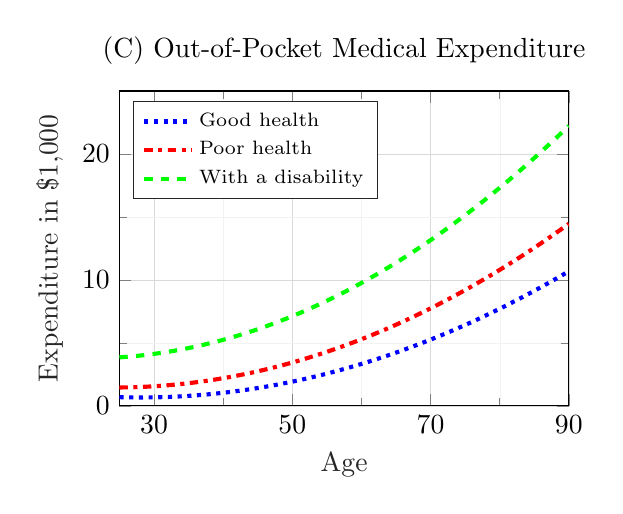
\begin{tikzpicture}
\begin{axis}[%
width=5.706cm,
height=4cm,
at={(0cm,0cm)},
scale only axis,
xmin=25,
xmax=90,
xtick={30,50,70,90},
xlabel style={font=\color{white!15!black}},
xlabel={Age},
ymin=0,
ymax=25,
ylabel style={font=\color{white!15!black}},
ylabel={Expenditure in \$1,000},
axis background/.style={fill=white},
%title style={font=\bfseries},
title={(C) Out-of-Pocket Medical Expenditure},
legend style={at={(axis cs:27,20.3)}, anchor=west, legend cell align=left, align=left, draw=white!15!black, font=\scriptsize},
grid=both,
grid style={line width=0.2pt, draw=gray!30},
minor grid style={line width=0.1pt, draw=gray!10},
minor tick num=1
]
% Blue line (h(t)=0) - dotted
\addplot [color=blue, line width=1.5pt, dotted]
  table[row sep=crcr]{%
25 0.69549069\\
26 0.68199083\\
27 0.67371464\\
28 0.6706623\\
29 0.67283363\\
30 0.68022881\\
31 0.69284784\\
32 0.71069035\\
33 0.73375671\\
34 0.76204674\\
35 0.79556062\\
36 0.83429816\\
37 0.87825956\\
38 0.92744462\\
39 0.98185335\\
40 1.04148593\\
41 1.10634236\\
42 1.17642228\\
43 1.25172585\\
44 1.33225347\\
45 1.41800457\\
46 1.5089797\\
47 1.60517831\\
48 1.70660078\\
49 1.81324709\\
50 1.92511801\\
51 2.04221129\\
52 2.16452841\\
53 2.29206939\\
54 2.42483423\\
55 2.56282291\\
56 2.70603545\\
57 2.85447183\\
58 3.00813021\\
59 3.1670143\\
60 3.33112225\\
61 3.50045404\\
62 3.67500783\\
63 3.85478546\\
64 4.03978882\\
65 4.23001602\\
66 4.42546521\\
67 4.62613826\\
68 4.83203516\\
69 5.0431559\\
70 5.25950051\\
71 5.48107082\\
72 5.70786313\\
73 5.93987742\\
74 6.17711743\\
75 6.41958129\\
76 6.667269\\
77 6.92017871\\
78 7.17831412\\
79 7.44167339\\
80 7.71025465\\
81 7.98406162\\
82 8.26309058\\
83 8.5473434\\
84 8.83682006\\
85 9.13152245\\
86 9.43144682\\
87 9.73659504\\
88 10.0469652\\
89 10.362563\\
90 10.6833828\\
};
\addlegendentry{Good health}

% Red line (h(t)=1) - dash-dotted
\addplot [color=red, line width=1.5pt, dashdotted]
  table[row sep=crcr]{%
25 1.46408419\\
26 1.47088973\\
27 1.48372673\\
28 1.50259464\\
29 1.52749401\\
30 1.55842446\\
31 1.59538601\\
32 1.63837884\\
33 1.68740294\\
34 1.74245794\\
35 1.8035444\\
36 1.87066252\\
37 1.94381135\\
38 2.02299071\\
39 2.10820247\\
40 2.19944476\\
41 2.29671758\\
42 2.40002279\\
43 2.50935854\\
44 2.62472481\\
45 2.74612348\\
46 2.87355268\\
47 3.00701427\\
48 3.14650454\\
49 3.29202905\\
50 3.44358224\\
51 3.60116782\\
52 3.76478393\\
53 3.93443244\\
54 4.11011148\\
55 4.29182105\\
56 4.47956301\\
57 4.6733355\\
58 4.87313852\\
59 5.07897394\\
60 5.29083989\\
61 5.50873637\\
62 5.73266525\\
63 5.96262465\\
64 6.19861645\\
65 6.44063878\\
66 6.68869164\\
67 6.94277503\\
68 7.20289082\\
69 7.46903714\\
70 7.74121585\\
71 8.01942509\\
72 8.30366486\\
73 8.59393703\\
74 8.89023973\\
75 9.19257296\\
76 9.50093858\\
77 9.81533473\\
78 10.1357614\\
79 10.4622205\\
80 10.7947101\\
81 11.1332302\\
82 11.4777846\\
83 11.8283658\\
84 12.1849813\\
85 12.5476292\\
86 12.9163038\\
87 13.2910127\\
88 13.6717522\\
89 14.0585203\\
90 14.4513245\\
};
\addlegendentry{Poor health}

% Green line (h(t)=2) - dashed
\addplot [color=green, line width=1.5pt, dashed]
  table[row sep=crcr]{%
25 3.85542075\\
26 3.89487722\\
27 3.94193474\\
28 3.99658957\\
29 4.05884358\\
30 4.12869677\\
31 4.20614726\\
32 4.29119694\\
33 4.38384579\\
34 4.48409196\\
35 4.5919373\\
36 4.70738183\\
37 4.83042552\\
38 4.9610684\\
39 5.09930859\\
40 5.24514795\\
41 5.3985865\\
42 5.55962235\\
43 5.72825925\\
44 5.90449346\\
45 6.08832499\\
46 6.27975755\\
47 6.47878743\\
48 6.68541649\\
49 6.89964472\\
50 7.12147213\\
51 7.35089685\\
52 7.58792075\\
53 7.83254383\\
54 8.08476422\\
55 8.34458379\\
56 8.61200254\\
57 8.88702046\\
58 9.16963756\\
59 9.45985011\\
60 9.7576637\\
61 10.0630765\\
62 10.3760884\\
63 10.6966977\\
64 11.0249061\\
65 11.3607119\\
66 11.7041168\\
67 12.0551246\\
68 12.4137279\\
69 12.7799285\\
70 13.1537301\\
71 13.5351272\\
72 13.9241253\\
73 14.3207226\\
74 14.7249191\\
75 15.1367111\\
76 15.5561059\\
77 15.983098\\
78 16.4176856\\
79 16.8598761\\
80 17.3096621\\
81 17.7670491\\
82 18.2320353\\
83 18.7046132\\
84 19.1848014\\
85 19.6725907\\
86 20.1679624\\
87 20.6709351\\
88 21.1815089\\
89 21.6997024\\
90 22.2254782\\
};
\addlegendentry{With a disability}
\end{axis}
\end{tikzpicture} & 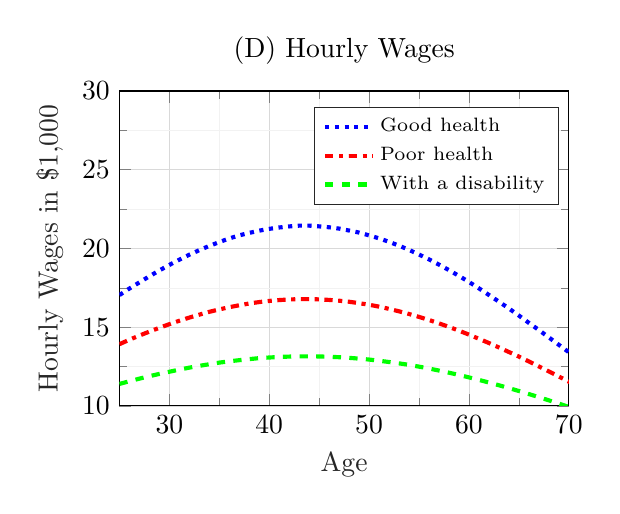
\begin{tikzpicture}
\begin{axis}[%
width=5.706cm,
height=4cm,
at={(0cm,0cm)},
scale only axis,
xmin=25,
xmax=70,
xlabel style={font=\color{white!15!black}},
xlabel={Age},
ymin=10,
ymax=30,
ylabel style={font=\color{white!15!black}},
ylabel={Hourly Wages in \$1,000},
axis background/.style={fill=white},
%title style={font=\bfseries},
title={(D) Hourly Wages},
legend style={at={(axis cs:69,29)}, anchor=north east, legend cell align=left, align=left, draw=white!15!black, font=\scriptsize},
grid=both,
grid style={line width=0.2pt, draw=gray!30},
minor grid style={line width=0.1pt, draw=gray!10},
minor tick num=1
]
% Blue line (h(t)=0) - dotted
\addplot [color=blue, line width=1.5pt, dotted]
  table[row sep=crcr]{%
25 17.038732931\\
26 17.4542862\\
27 17.8458896\\
28 18.2333825\\
29 18.6034326\\
30 18.9545214\\
31 19.2874174\\
32 19.6000282\\
33 19.8910738\\
34 20.1595058\\
35 20.4032752\\
36 20.6349778\\
37 20.8299873\\
38 20.9875306\\
39 21.1294096\\
40 21.2430726\\
41 21.3293168\\
42 21.3971419\\
43 21.4465891\\
44 21.4472714\\
45 21.4000386\\
46 21.3431199\\
47 21.2595208\\
48 21.1359871\\
49 21.0057627\\
50 20.8289922\\
51 20.6396637\\
52 20.4187952\\
53 20.1755905\\
54 19.9054845\\
55 19.6151301\\
56 19.3050955\\
57 18.9731394\\
58 18.6231478\\
59 18.2534162\\
60 17.8725251\\
61 17.4667029\\
62 17.0430688\\
63 16.6240313\\
64 16.1871244\\
65 15.7395087\\
66 15.2739585\\
67 14.8207176\\
68 14.3532838\\
69 13.8810528\\
70 13.4097773\\
71 12.9349057\\
72 12.4596877\\
73 11.9863954\\
74 11.5156889\\
75 11.0495625\\
76 10.5862582\\
77 10.1178357\\
78 9.6800105\\
79 9.2399334\\
80 8.8042616\\
81 8.3797474\\
82 7.9649453\\
83 7.5606193\\
84 7.1672203\\
85 6.7840423\\
86 6.4149422\\
87 6.0569024\\
88 5.7111602\\
89 5.3778823\\
90 5.0573577\\
};
\addlegendentry{Good health}

% Red line (h(t)=1) - dash-dotted
\addplot [color=red, line width=1.5pt, dashdotted]
  table[row sep=crcr]{%
25 13.9207948\\
26 14.2047403\\
27 14.4674653\\
28 14.7182134\\
29 14.9623434\\
30 15.1910459\\
31 15.4087123\\
32 15.6087075\\
33 15.7961556\\
34 15.9738525\\
35 16.1282511\\
36 16.2684047\\
37 16.3923221\\
38 16.5039362\\
39 16.5943431\\
40 16.6654026\\
41 16.7207774\\
42 16.7588626\\
43 16.7789271\\
44 16.7809953\\
45 16.7649334\\
46 16.7304199\\
47 16.6802994\\
48 16.6140951\\
49 16.5227746\\
50 16.4246175\\
51 16.3035138\\
52 16.1600103\\
53 16.0063856\\
54 15.8372274\\
55 15.6530267\\
56 15.4545121\\
57 15.2417903\\
58 15.0159812\\
59 14.7776676\\
60 14.5274988\\
61 14.2621611\\
62 13.9945643\\
63 13.7143475\\
64 13.4233456\\
65 13.1343654\\
66 12.8222313\\
67 12.5077179\\
68 12.1916875\\
69 11.8699484\\
70 11.5442478\\
71 11.2153607\\
72 10.8822157\\
73 10.5514423\\
74 10.2179713\\
75 9.8842727\\
76 9.5512479\\
77 9.2185561\\
78 8.8888729\\
79 8.5626167\\
80 8.2386738\\
81 7.9184131\\
82 7.6024837\\
83 7.2932698\\
84 6.9862644\\
85 6.6848614\\
86 6.3906564\\
87 6.0569024\\
88 5.7111602\\
89 5.3778823\\
90 5.0573577\\
};
\addlegendentry{Poor health}

% Green line (h(t)=2) - dashed
\addplot [color=green, line width=1.5pt, dashed]
  table[row sep=crcr]{%
25 11.3963276\\
26 11.5667395\\
27 11.7321955\\
28 11.8862335\\
29 12.0326526\\
30 12.1689006\\
31 12.3078104\\
32 12.4301344\\
33 12.5440848\\
34 12.6468777\\
35 12.7489912\\
36 12.8328886\\
37 12.9037903\\
38 12.9716965\\
39 13.0340029\\
40 13.0733775\\
41 13.1080689\\
42 13.1321171\\
43 13.1455988\\
44 13.1483318\\
45 13.1403785\\
46 13.1218273\\
47 13.0926326\\
48 13.0528585\\
49 13.0016644\\
50 12.9431201\\
51 12.8703837\\
52 12.7866147\\
53 12.7004345\\
54 12.6064182\\
55 12.4933071\\
56 12.3756657\\
57 12.2442144\\
58 12.1086155\\
59 11.9659139\\
60 11.8118108\\
61 11.6521229\\
62 11.4852695\\
63 11.3116547\\
64 11.1304946\\
65 10.9473952\\
66 10.7536501\\
67 10.5566969\\
68 10.354914\\
69 10.1486702\\
70 9.9385408\\
71 9.7247835\\
72 9.5079214\\
73 9.2853921\\
74 9.0644669\\
75 8.8426994\\
76 8.6174101\\
77 8.3910749\\
78 8.1640136\\
79 7.9366855\\
80 7.7074157\\
81 7.4825711\\
82 7.2584391\\
83 7.0344812\\
84 6.8119217\\
85 6.5861317\\
86 6.3664108\\
87 6.0569024\\
88 5.7111602\\
89 5.3778823\\
90 5.0573577\\
};
\addlegendentry{With a disability}
\end{axis}
\end{tikzpicture}
\end{tabular}
\tabnotes{\textit{Notes:} Panel A shows the probability of being in good health, in poor health, or with a disability at age $t+1$ for an individual in good health at age $t$. Panel B shows annual mortality rates (percent), panel C annual out-of-pocket medical expenditures (thousands of dollars), and panel D offered hourly wages corrected for selection (dollars), by age and health status. Blue dotted, red dash-dotted, and green dashed lines refer to good health, poor health, and disability. Monetary values are in 2016 dollars. \textit{Data sources:} Panel Study of Income Dynamics (panels A, B, and D) and Medical Expenditure Panel Survey (panel C).}
\end{figure}

\begin{table}[!htbp]
\centering
\caption{First-Step and Calibrated Parameters}\label{tab:calibrated}
\small
% Table body for tab:calibrated (Section 3).
% Sources: FROT tables/parameters_summary.tex (rho = 0.981, sigma^2 = 0.016, ERA 62, NRA 65, DRC 4.5%; scratchpad src/tables/parameters_summary.tex);
% r_f = 4%, 20% wedge, consumption floor $3,500: FROT 2025_sub/5_quantitative_model.tex (First-Step Estimation) and blueprint Sec. 5; floor attribution corrected to French2004.
\begin{tabular}{@{}l l l l@{}}
\toprule
Parameter & Description & Value & Source \\
\midrule
\multicolumn{4}{@{}l}{\textit{A. Estimated from data outside the model}} \\
$\pi_{j,i,t+1}$ & Health transition probabilities & Fig.~\ref{fig:firststep}A & PSID \\
$S(h,t)$ & Survival probabilities & Fig.~\ref{fig:firststep}B & PSID \\
$M(h,t,P)$ & Out-of-pocket medical expenses & Fig.~\ref{fig:firststep}C & MEPS \\
$W(h,t)$ & Deterministic wage profiles & Fig.~\ref{fig:firststep}D & PSID \\
$\rho$ & Autocorrelation of log ability & 0.981 & PSID \\
$\sigma^2$ & Variance of ability innovations & 0.016 & PSID \\
$\lambda_t,\tau_t$ & Income tax function by age & Age-specific & \citet{Borella2023} \\
\addlinespace
\multicolumn{4}{@{}l}{\textit{B. Taken from the literature}} \\
% AUTHORS: the r_f (French 2005) and tau_k (Stantcheva 2017) attributions follow FROT 2025_sub/5_quantitative_model.tex; a reviewer could not locate either value in the cited papers. Add page/table references or cite the original sources.
$r_f$ & Gross interest rate & 4\% & \citet{french2005effects} \\
$\tau_k$ & Wedge between gross and net return & 20\% & \citet{Stantcheva2017} \\
$\underline{c}$ & Consumption floor & \$3,500 & \citet{French2004} \\ % Attribution per verified_facts item 8: $3,500 is French and Jones (2004, CRR WP 2004-12), not French and Jones (2011).
\addlinespace
\multicolumn{4}{@{}l}{\textit{C. Program rules, cohorts born 1920--1940}} \\
ERA & Early retirement age & 62 & SSA \\
NRA & Normal retirement age & 65 & SSA \\
DRC & Delayed retirement credit & 4.5\% & SSA \\
 & Other Social Security rules & Table~\ref{tab:ssparams} & SSA \\
\bottomrule
\end{tabular}

\tabnotes{\textit{Notes:} Parameters fixed before the second-step estimation. Panel A lists objects estimated directly from the data (Appendix~\ref{app:firststep}); $\rho$ and $\sigma^2$ are the autocorrelation and innovation variance of log ability $\ln\theta_t$; the income tax function $T_t(y)=y-\lambda_t y^{1-\tau_t}$ is estimated by age following \citet{Borella2023}. Panel B lists values taken from earlier studies; the net return on savings is $r=(1-\tau_k)r_f=3.2\%$. Panel C lists Social Security rules for the 1920--1940 birth cohorts; the DRC is the cohort average of credits that varied with the year of birth. Abbreviations: ERA, early retirement age; NRA, normal retirement age; DRC, delayed retirement credit; PSID, Panel Study of Income Dynamics; MEPS, Medical Expenditure Panel Survey; SSA, Social Security Administration.}
\end{table}

\subsection{Second-Step Estimation by the Method of Simulated Moments}

\paragraph{Moments and criterion.} For each age from 30 to 69 ($T=40$ ages), we match seven moments: the participation rates of healthy and unhealthy individuals, the mean annual hours of healthy and unhealthy participants, mean and median nonpension assets, and the mean reentry rate. This yields $7\times 40=280$ moment conditions. Because the labor-supply moments pool poor health and disability, the two states share a fixed cost of participation, $\phi_n(1)=\phi_n(2)$.

Let $\hat{\varphi}(\mathcal{P};\chi)$ denote the 280-element vector of differences between the data moments and the corresponding moments of the model, simulated from the decision rules (Appendix~\ref{app:solution}) for individuals who start from the empirical distribution of initial conditions and draw health, survival, and wage shocks from the first-step processes. The MSM estimator is
\[
\hat{\mathcal{P}}=\argmin_{\mathcal{P}}\ \frac{N}{1+N/N_s}\ \hat{\varphi}(\mathcal{P};\chi)'\,\hat{\mathbf{W}}\,\hat{\varphi}(\mathcal{P};\chi),
\]
where $N$ is the number of observations in the data, $N_s$ is the number of simulated observations, and the factor $1+N/N_s$ accounts for simulation error. The weighting matrix $\hat{\mathbf{W}}$ is the inverse of a diagonal matrix that holds the sampling variances of the data moments, so each moment is weighted by its precision. Appendix~\ref{app:msm} lists the moment conditions and the estimation algorithm and derives the standard errors.

\paragraph{Identification.} As in \citet{french2005effects}, identification rests on two assumptions: work decisions do not affect health or wages, and age shifts the incentives to work and save---through wages, health, mortality, medical expenses, and the rules of Social Security and pensions---but not preferences. Under these assumptions, the first step measures how incentives change with age and health, and the behavior that these incentives do not explain identifies preferences. The discount factor $\beta$ is identified by intertemporal substitution, and hence by the asset and labor-supply profiles, especially at the ages at which individuals accumulate wealth for retirement. The time endowment $L$ and the fixed costs $\phi_n(h)$ are identified by participation and hours by health status: with a fixed cost, individuals either work substantial hours or do not work at all, so the participation rate and the hours of those who work carry separate information, and the gap between the participation profiles of healthy and unhealthy individuals, given their first-step wages and medical costs, pins down the health gradient in the fixed cost. The reentry cost $\phi_{RE}$ is identified by the low reentry rates in the data. The curvature parameters $\nu$ and $\gamma$ are identified by the asset and labor-supply profiles: higher risk aversion raises precautionary saving and encourages more work earlier in life.

\subsection{Parameter Estimates}

\autoref{tab:estimates} reports the estimates. The discount factor is 0.98. The annual time endowment is 4,491 hours, and the fixed cost of working is 791 hours for healthy individuals and 868 hours for individuals in poor health or with a disability. A healthy participant thus gives up about 18 percent of her time endowment before working the first hour, and an unhealthy participant about 19 percent (ratios of the table entries, $791.07/4490.5$ and $867.54/4490.5$). This nonconvexity is what makes retirement a discrete decision in the model: workers choose between substantial hours and full exit, so a reform moves labor supply mainly by changing the age of exit. The health gradient in the fixed cost compounds the lower wages, higher medical expenses, and access to DI of unhealthy individuals, each of which also pulls their exit forward. The time endowment and the fixed costs fall within the range of estimates in \citet{french2011effects} and \citet{Borella2023}.

The reentry cost is 3,312 hours, about three-quarters of the annual time endowment (the ratio $3311.5/4490.5$). Leaving the labor force is therefore close to irreversible, and a reform that encourages later retirement acts on workers before they exit rather than drawing retirees back into work.

The curvature of flow utility is $\nu=1.70$ and the consumption weight is $\gamma=0.54$, which imply a coefficient of relative risk aversion over consumption, $-u_{cc}c/u_c=1-\gamma(1-\nu)$, of approximately 1.38. Because $\nu>1$, the marginal utility of consumption falls as leisure rises, so consumption optimally declines at retirement. The two parameters also scale the consumption-equivalent welfare measure of Section~\ref{sec:fw_welfare}, which converts changes in expected utility into changes in consumption through $\gamma(1-\nu)$.

The overidentification statistic is 1463 with $280-7=273$ degrees of freedom, so the test formally rejects the model, as in earlier studies that estimate life-cycle retirement models on many precisely measured moments \citep{french2005effects,french2011effects}. The test asks the model to match 280 profiles at every age within sampling error; the relevant question for our purposes is whether it reproduces the patterns of labor supply and saving through which retirement reforms operate, to which we now turn.

\begin{table}[!htbp]
\centering
\caption{Estimated Preference Parameters}\label{tab:estimates}
\small
% Table body for tab:estimates (Section 3).
% Source: FROT tables/estimated_parameters.tex (scratchpad copy: src/tables/estimated_parameters.tex).
% Every estimate, standard error, and the chi-square statistic is copied exactly; rows regrouped only.
\begin{tabular}{@{}l l r r@{}}
\toprule
Parameter & Description & Estimate & Std.\ error \\
\midrule
\multicolumn{4}{@{}l}{\textit{Preferences}} \\
$\gamma$ & Consumption weight & 0.5354 & 0.0047 \\
$\nu$ & Curvature of the consumption--leisure composite & 1.7029 & 0.0681 \\
$\beta$ & Time discount factor & 0.9797 & 0.0023 \\
\addlinespace
\multicolumn{4}{@{}l}{\textit{Time endowment and time costs (hours per year)}} \\
$L$ & Time endowment & 4490.5 & 21.65 \\
$\phi_n(0)$ & Fixed cost of work, good health & 791.07 & 15.65 \\
$\phi_n(1)=\phi_n(2)$ & Fixed cost of work, poor health or disability & 867.54 & 22.68 \\
$\phi_{RE}$ & Labor market reentry cost & 3311.5 & 82.02 \\
\midrule
\multicolumn{2}{@{}l}{Overidentification statistic, $\chi^2$ (273 degrees of freedom)} & 1463 & \\
\bottomrule
\end{tabular}

\tabnotes{\textit{Notes:} Method-of-simulated-moments estimates of the preference parameters and their asymptotic standard errors (Appendix~\ref{app:msm}). $\gamma$ is the weight on consumption and $\nu$ the curvature in $u(c,l)=(c^{\gamma}l^{1-\gamma})^{1-\nu}/(1-\nu)$; the implied relative risk aversion over consumption is $1-\gamma(1-\nu)\approx1.38$. $L$, $\phi_n(h)$, and $\phi_{RE}$ are measured in hours per year; poor health ($h=1$) and disability ($h=2$) share one fixed cost of work. The overidentification statistic tests the 280 moment conditions against 7 parameters. \textit{Data source:} Panel Study of Income Dynamics.}
\end{table}

\subsection{Match of Moments}

\autoref{fig:fit_labor} compares the simulated profiles of participation and hours with their PSID counterparts and 95 percent confidence intervals. In the data, participation is high and stable in the 30s and 40s, declines from the early 50s for individuals in poor health or with a disability, and drops sharply in the 60s in both health groups. These declines coincide with falling wages and with growing retirement incentives from pensions and Social Security. The model reproduces these patterns. As emphasized by \citet{Yu2024}, the explicit disability state and DI benefits are essential for the decline in the participation of unhealthy individuals from their 50s: DI provides an alternative pathway out of the labor force for people with a disability \citep{Maestas2013,French2014,Low2015,Li2018}, and modeling it yields a closer fit for this group than in earlier work such as \citet{french2005effects}.

The departures are informative about where the model is weakest. For unhealthy individuals, the model overstates participation in the 40s and concentrates the decline at age 50, the age from which DI is available in the model, whereas the decline in the data is spread over the late 40s and early 50s. Between the late 50s and the mid-60s, simulated participation of the unhealthy lies at or below the lower bound of the confidence band, and simulated participation of the healthy lies slightly below the data around age 60: simulated exit is somewhat early. Hours of participants decline in the 60s in the model as in the data, but the model places the hours of unhealthy workers, and to a lesser extent those of healthy workers, below the data before age 60.

The fit of unhealthy participation between 55 and 69 matters for the reform analysis because these are the ages at which three exit routes compete for the same individuals: DI, which pays the primary insurance amount without an early-claiming reduction until the NRA; early claiming of reduced retirement benefits from age 62; and continued work. Claiming-age reforms shift the relative value of these routes. Raising the NRA lowers retirement benefits at every claiming age while extending the ages at which DI is paid; raising the DRC increases the reward for delay, which individuals with higher mortality value less. The resulting reallocation across programs is what the indirect fiscal effects of Section~\ref{sec:framework} measure. Because simulated exit of the unhealthy is somewhat early, the model, if anything, places fewer unhealthy workers at the margin between work and claiming at ages 62 to 64 than the data do.

\begin{figure}[!htbp]
\centering
\caption{Data and Simulated Profiles: Participation and Hours}\label{fig:fit_labor}
\vspace{0.5em}
% Fit panels: corrected 2026 re-simulation of the estimated model at the same estimates (FROT figures/abdou/*_c.tex), copied verbatim.
\begin{tabular}{@{}c@{\hspace{1.5em}}c@{}}
\begin{tikzpicture}
\begin{axis}[%
width=5.706cm,
height=4cm,
at={(0cm,0cm)},
scale only axis,
xmin=30,
xmax=70,
xlabel style={font=\color{white!15!black}},
xlabel={Age},
ymin=-5,
ymax=100,
ylabel style={font=\color{white!15!black}},
ylabel={Rate in \%},
axis background/.style={fill=white},
%title style={font=\bfseries},
title={(A) Healthy Labor Force Participation Rate},
legend style={at={(axis cs:32,0)}, anchor=south west, legend cell align=left, align=left, draw=white!15!black, font=\scriptsize},
grid=both,
grid style={line width=0.2pt, draw=gray!30},
minor grid style={line width=0.1pt, draw=gray!10},
minor tick num=1
]

% Main line (lfprlr0) - blue solid line
\addplot [color=black, line width=1pt]
  table[row sep=crcr, y expr=\thisrowno{1}*100]{%
30 0.8833822\\
31 0.8728638\\
32 0.8650124\\
33 0.8656822\\
34 0.8743696\\
35 0.873809\\
36 0.8829339\\
37 0.8818902\\
38 0.8847443\\
39 0.8934818\\
40 0.8900082\\
41 0.8684802\\
42 0.8632262\\
43 0.8659114\\
44 0.8597141\\
45 0.8664337\\
46 0.866869\\
47 0.8677746\\
48 0.8541223\\
49 0.8445035\\
50 0.8394285\\
51 0.8343548\\
52 0.8268231\\
53 0.8226036\\
54 0.8069361\\
55 0.7833442\\
56 0.7647346\\
57 0.7266455\\
58 0.7198906\\
59 0.6746376\\
60 0.6433743\\
61 0.5887213\\
62 0.4924323\\
63 0.4207888\\
64 0.3610537\\
65 0.2870897\\
66 0.2260264\\
67 0.21724\\
68 0.1962348\\
69 0.1569484\\
% 70 0.1681354\\
% 71 0.121358\\
% 72 0.1394618\\
% 73 0.1092736\\
% 74 0.1141775\\
% 75 0.0792269\\
% 76 0.0917666\\
% 77 0.0850947\\
% 78 0.0388536\\
% 79 0.0336195\\
% 80 0.058109\\
% 81 0.016314\\
% 82 0.0270162\\
% 83 -0.0089496\\
% 84 0.0236253\\
% 85 -0.0178846\\
};
\addlegendentry{Data}

% Upper bound (standard error high)
\addplot[name path=upper, draw=none, forget plot] 
  table[row sep=crcr,y expr=\thisrowno{1}*100]{%
30 0.9051051\\
31 0.8935855\\
32 0.8848711\\
33 0.88477\\
34 0.892873\\
35 0.8917789\\
36 0.9007229\\
37 0.8994025\\
38 0.9019169\\
39 0.9103903\\
40 0.9066504\\
41 0.8923349\\
42 0.8859496\\
43 0.8876875\\
44 0.8808528\\
45 0.8869151\\
46 0.88653\\
47 0.8869081\\
48 0.8729149\\
49 0.863117\\
50 0.858066\\
51 0.8529794\\
52 0.8455561\\
53 0.8413141\\
54 0.8257702\\
55 0.8021987\\
56 0.7835673\\
57 0.7460628\\
58 0.739598\\
59 0.6947576\\
60 0.663489\\
61 0.6094228\\
62 0.5136542\\
63 0.4426488\\
64 0.3833388\\
65 0.3098885\\
66 0.2493425\\
67 0.2413235\\
68 0.2207975\\
69 0.1832494\\
% 70 0.194256\\
% 71 0.1491448\\
% 72 0.1675596\\
% 73 0.1396055\\
% 74 0.1450964\\
% 75 0.1120739\\
% 76 0.1273876\\
% 77 0.1228318\\
% 78 0.0783176\\
% 79 0.0761687\\
% 80 0.1034711\\
% 81 0.0718914\\
% 82 0.080405\\
% 83 0.0504064\\
% 84 0.082339\\
% 85 0.0525297\\
};

% Lower bound (standard error low)
\addplot[name path=lower, draw=none, forget plot] 
  table[row sep=crcr,y expr=\thisrowno{1}*100]{%
30 0.8616592\\
31 0.852142\\
32 0.8451536\\
33 0.8465945\\
34 0.8558661\\
35 0.855839\\
36 0.8651446\\
37 0.8643779\\
38 0.8675715\\
39 0.8765733\\
40 0.8733659\\
41 0.8446254\\
42 0.8405027\\
43 0.8441353\\
44 0.8385755\\
45 0.8459523\\
46 0.8472079\\
47 0.848641\\
48 0.8353298\\
49 0.8258898\\
50 0.8207909\\
51 0.81573\\
52 0.80809\\
53 0.8038934\\
54 0.788102\\
55 0.7644898\\
56 0.7459021\\
57 0.7072282\\
58 0.7001832\\
59 0.6545175\\
60 0.6232595\\
61 0.5680198\\
62 0.4712104\\
63 0.3989288\\
64 0.3387687\\
65 0.2642909\\
66 0.2027102\\
67 0.1931565\\
68 0.1716722\\
69 0.1306474\\
% 70 0.1420148\\
% 71 0.0935712\\
% 72 0.111364\\
% 73 0.0789419\\
% 74 0.0832585\\
% 75 0.04638\\
% 76 0.0561455\\
% 77 0.0473576\\
% 78 -0.0006104\\
% 79 -0.0089297\\
% 80 0.012747\\
% 81 -0.0392634\\
% 82 -0.0263728\\
% 83 -0.0683057\\
% 84 -0.0350885\\
% 85 -0.0882989\\
};

% Fill between the paths
\addplot[blue!30] fill between[of=upper and lower];
\addlegendentry{95\% C.I.}

\addplot [color=red, line width=1.5pt, dashed]
  table[row sep=crcr,y expr=\thisrowno{1}*100]{%
30	0.932489451	\\
31	0.926638605	\\
32	0.921274038	\\
33	0.914777879	\\
34	0.910546993	\\
35	0.908122908	\\
36	0.906507791	\\
37	0.900768049	\\
38	0.898980538	\\
39	0.892446379	\\
40	0.889968652	\\
41	0.890397979	\\
42	0.886493342	\\
43	0.882240611	\\
44	0.877681716	\\
45	0.872236671	\\
46	0.868164063	\\
47	0.864026403	\\
48	0.85709527	\\
49	0.855082187	\\
50	0.850991114	\\
51	0.842930153	\\
52	0.831024931	\\
53	0.820189274	\\
54	0.805821796	\\
55	0.775583483	\\
56	0.751822157	\\
57	0.725018505	\\
58	0.69141791	\\
59	0.654428463	\\
60	0.591907514	\\
61	0.528448948	\\
62	0.460984394	\\
63	0.39049167	\\
64	0.335378323	\\
65	0.272953885	\\
66	0.210012728	\\
67	0.162587413	\\
68	0.141104294	\\
69	0.118198037	\\
  };
\addlegendentry{Model}

\end{axis}
\end{tikzpicture} & \begin{tikzpicture}
\begin{axis}[%
width=5.706cm,
height=4cm,
at={(0cm,0cm)},
scale only axis,
xmin=30,
xmax=70,
xlabel style={font=\color{white!15!black}},
xlabel={Age},
ymin=-5,
ymax=100,
ylabel style={font=\color{white!15!black}},
ylabel={Rate in \%},
axis background/.style={fill=white},
%title style={font=\bfseries},
title={(B) Unhealthy Labor Force Participation Rate},
legend style={at={(axis cs:32,0)}, anchor=south west, legend cell align=left, align=left, draw=white!15!black, font=\scriptsize},
grid=both,
grid style={line width=0.2pt, draw=gray!30},
minor grid style={line width=0.1pt, draw=gray!10},
minor tick num=1
]

% Main line (lfprlr0) - blue solid line
\addplot [color=black, line width=1pt]
  table[row sep=crcr,y expr=\thisrowno{1}*100]{%
30 0.8339695\\
31 0.830355\\
32 0.8042343\\
33 0.7983715\\
34 0.7995418\\
35 0.8378634\\
36 0.8354884\\
37 0.8686402\\
38 0.8411449\\
39 0.8375973\\
40 0.8386171\\
41 0.8234905\\
42 0.8157026\\
43 0.7707186\\
44 0.7771355\\
45 0.7791017\\
46 0.7758368\\
47 0.7928331\\
48 0.762918\\
49 0.710295\\
50 0.6906397\\
51 0.6569952\\
52 0.6095482\\
53 0.5680759\\
54 0.5703449\\
55 0.5509109\\
56 0.5310219\\
57 0.5219091\\
58 0.4718995\\
59 0.4247883\\
60 0.4079395\\
61 0.3693248\\
62 0.2990521\\
63 0.2519826\\
64 0.2448949\\
65 0.1944834\\
66 0.1670593\\
67 0.1475739\\
68 0.1256826\\
69 0.1083655\\
% 70 0.1681354\\
% 71 0.121358\\
% 72 0.1394618\\
% 73 0.1092736\\
% 74 0.1141775\\
% 75 0.0792269\\
% 76 0.0917666\\
% 77 0.0850947\\
% 78 0.0388536\\
% 79 0.0336195\\
% 80 0.058109\\
% 81 0.016314\\
% 82 0.0270162\\
% 83 -0.0089496\\
% 84 0.0236253\\
% 85 -0.0178846\\
};
\addlegendentry{Data}

% Upper bound (standard error high)
\addplot[name path=upper, draw=none, forget plot] 
  table[row sep=crcr,y expr=\thisrowno{1}*100]{%
30 0.9111052\\
31 0.9001306\\
32 0.8669667\\
33 0.8606798\\
34 0.860257\\
35 0.8955216\\
36 0.8874309\\
37 0.9166927\\
38 0.8892378\\
39 0.8830312\\
40 0.8826435\\
41 0.8928777\\
42 0.8792804\\
43 0.8314206\\
44 0.83197\\
45 0.8315616\\
46 0.8263692\\
47 0.8398106\\
48 0.8062539\\
49 0.7522238\\
50 0.7306355\\
51 0.6956045\\
52 0.6471571\\
53 0.6047442\\
54 0.6048974\\
55 0.5855613\\
56 0.5653728\\
57 0.5550599\\
58 0.5043322\\
59 0.4570315\\
60 0.4391904\\
61 0.4005467\\
62 0.3297285\\
63 0.2832072\\
64 0.2764793\\
65 0.2267636\\
66 0.1990062\\
67 0.1796762\\
68 0.1588332\\
69 0.142154\\
% 70 0.194256\\
% 71 0.1491448\\
% 72 0.1675596\\
% 73 0.1396055\\
% 74 0.1450964\\
% 75 0.1120739\\
% 76 0.1273876\\
% 77 0.1228318\\
% 78 0.0783176\\
% 79 0.0761687\\
% 80 0.1034711\\
% 81 0.0718914\\
% 82 0.080405\\
% 83 0.0504064\\
% 84 0.082339\\
% 85 0.0525297\\
};

% Lower bound (standard error low)
\addplot[name path=lower, draw=none, forget plot] 
  table[row sep=crcr,y expr=\thisrowno{1}*100]{%
30 0.7568338\\
31 0.7605796\\
32 0.7415019\\
33 0.7360631\\
34 0.7388266\\
35 0.7802051\\
36 0.7835459\\
37 0.8205878\\
38 0.7930518\\
39 0.7921634\\
40 0.7945906\\
41 0.7541034\\
42 0.7521245\\
43 0.7100167\\
44 0.7223011\\
45 0.7266418\\
46 0.7253045\\
47 0.7458558\\
48 0.719582\\
49 0.6683661\\
50 0.6506439\\
51 0.618386\\
52 0.5719393\\
53 0.5314076\\
54 0.5357924\\
55 0.5162606\\
56 0.496671\\
57 0.4887584\\
58 0.4394668\\
59 0.3925449\\
60 0.3766887\\
61 0.3381029\\
62 0.2683756\\
63 0.2207581\\
64 0.2133105\\
65 0.1622031\\
66 0.1351124\\
67 0.1154717\\
68 0.092532\\
69 0.0745769\\
% 70 0.1420148\\
% 71 0.0935712\\
% 72 0.111364\\
% 73 0.0789419\\
% 74 0.0832585\\
% 75 0.04638\\
% 76 0.0561455\\
% 77 0.0473576\\
% 78 -0.0006104\\
% 79 -0.0089297\\
% 80 0.012747\\
% 81 -0.0392634\\
% 82 -0.0263728\\
% 83 -0.0683057\\
% 84 -0.0350885\\
% 85 -0.0882989\\
};

% Fill between the paths
\addplot[blue!30] fill between[of=upper and lower];
\addlegendentry{95\% C.I.}

\addplot [color=red, line width=1.5pt, dashed]
  table[row sep=crcr,y expr=\thisrowno{1}*100]{%
30	0.78021978	\\
31	0.75862069	\\
32	0.755813953	\\
33	0.816753927	\\
34	0.832460733	\\
35	0.835680751	\\
36	0.841409692	\\
37	0.873469388	\\
38	0.863117871	\\
39	0.897526502	\\
40	0.877419355	\\
41	0.853293413	\\
42	0.838150289	\\
43	0.840782123	\\
44	0.840848806	\\
45	0.856132075	\\
46	0.845794393	\\
47	0.84893617	\\
48	0.857429719	\\
49	0.849710983	\\
50	0.724738676	\\
51	0.642477876	\\
52	0.602941176	\\
53	0.557959815	\\
54	0.509516837	\\
55	0.490909091	\\
56	0.468253968	\\
57	0.441102757	\\
58	0.396341463	\\
59	0.378787879	\\
60	0.298342541	\\
61	0.263383298	\\
62	0.225774226	\\
63	0.200192493	\\
64	0.178199052	\\
65	0.154620311	\\
66	0.133858268	\\
67	0.122937294	\\
68	0.087027915	\\
69	0.082670906	\\
  };
\addlegendentry{Model}

\end{axis}
\end{tikzpicture} \\[1ex]
\begin{tikzpicture}
\begin{axis}[%
width=5.706cm,
height=4cm,
at={(0cm,0cm)},
scale only axis,
xmin=30,
xmax=70,
xlabel style={font=\color{white!15!black}},
xlabel={Age},
ymin=-100,
ymax=2500,
ylabel style={font=\color{white!15!black}},
ylabel={Hours in a Year},
axis background/.style={fill=white},
%title style={font=\bfseries},
title={(C) Hours Worked of Healthy},
legend style={at={(axis cs:32,0)}, anchor=south west, legend cell align=left, align=left, draw=white!15!black, font=\scriptsize},
grid=both,
grid style={line width=0.2pt, draw=gray!30},
minor grid style={line width=0.1pt, draw=gray!10},
minor tick num=1
]

% Main line (lfprlr0) - blue solid line
\addplot [color=black, line width=1pt]
  table[row sep=crcr]{%
30 2143.776\\
31 2139.441\\
32 2143.99\\
33 2145.759\\
34 2139.533\\
35 2148.389\\
36 2139.108\\
37 2131.988\\
38 2146.241\\
39 2150.673\\
40 2152.556\\
41 2110.49\\
42 2149.378\\
43 2124.506\\
44 2138.751\\
45 2125.451\\
46 2126.24\\
47 2100.008\\
48 2092.962\\
49 2066.729\\
50 2072.279\\
51 2062.416\\
52 2068.127\\
53 2049.428\\
54 2061.603\\
55 2035.663\\
56 2019.648\\
57 2005.664\\
58 1970.462\\
59 1973.028\\
60 1938.318\\
61 1903.091\\
62 1804.867\\
63 1795.704\\
64 1651.485\\
65 1601.154\\
66 1609.429\\
67 1459.81\\
68 1414.398\\
69 1453.738\\
% 70 0.1681354\\
% 71 0.121358\\
% 72 0.1394618\\
% 73 0.1092736\\
% 74 0.1141775\\
% 75 0.0792269\\
% 76 0.0917666\\
% 77 0.0850947\\
% 78 0.0388536\\
% 79 0.0336195\\
% 80 0.058109\\
% 81 0.016314\\
% 82 0.0270162\\
% 83 -0.0089496\\
% 84 0.0236253\\
% 85 -0.0178846\\
};
\addlegendentry{Data}

% Upper bound (standard error high)
\addplot[name path=upper, draw=none, forget plot] 
  table[row sep=crcr]{%
30 2178.159\\
31 2172.766\\
32 2176.314\\
33 2177.107\\
34 2170.112\\
35 2178.354\\
36 2168.583\\
37 2161.071\\
38 2174.72\\
39 2178.67\\
40 2180.178\\
41 2149.47\\
42 2186.848\\
43 2160.524\\
44 2174.171\\
45 2159.688\\
46 2159.397\\
47 2132.224\\
48 2125.058\\
49 2098.81\\
50 2104.721\\
51 2095.058\\
52 2101.074\\
53 2082.783\\
54 2095.726\\
55 2070.287\\
56 2054.273\\
57 2042.598\\
58 2008.204\\
59 2012.989\\
60 1978.96\\
61 1946.624\\
62 1853.525\\
63 1850.296\\
64 1710.904\\
65 1670.316\\
66 1684.934\\
67 1544.774\\
68 1499.869\\
69 1563.532\\
% 70 0.194256\\
% 71 0.1491448\\
% 72 0.1675596\\
% 73 0.1396055\\
% 74 0.1450964\\
% 75 0.1120739\\
% 76 0.1273876\\
% 77 0.1228318\\
% 78 0.0783176\\
% 79 0.0761687\\
% 80 0.1034711\\
% 81 0.0718914\\
% 82 0.080405\\
% 83 0.0504064\\
% 84 0.082339\\
% 85 0.0525297\\
};

% Lower bound (standard error low)
\addplot[name path=lower, draw=none, forget plot] 
  table[row sep=crcr]{%
30 2109.393\\
31 2106.114\\
32 2111.666\\
33 2114.411\\
34 2108.954\\
35 2118.425\\
36 2109.633\\
37 2102.906\\
38 2117.763\\
39 2122.676\\
40 2124.933\\
41 2071.511\\
42 2111.908\\
43 2088.489\\
44 2103.332\\
45 2091.215\\
46 2093.082\\
47 2067.791\\
48 2060.867\\
49 2034.649\\
50 2039.836\\
51 2029.775\\
52 2035.18\\
53 2016.075\\
54 2027.478\\
55 2001.039\\
56 1985.023\\
57 1968.731\\
58 1932.72\\
59 1933.067\\
60 1897.676\\
61 1859.56\\
62 1756.209\\
63 1741.111\\
64 1592.067\\
65 1531.993\\
66 1533.925\\
67 1374.848\\
68 1328.928\\
69 1343.943\\
% 70 0.1420148\\
% 71 0.0935712\\
% 72 0.111364\\
% 73 0.0789419\\
% 74 0.0832585\\
% 75 0.04638\\
% 76 0.0561455\\
% 77 0.0473576\\
% 78 -0.0006104\\
% 79 -0.0089297\\
% 80 0.012747\\
% 81 -0.0392634\\
% 82 -0.0263728\\
% 83 -0.0683057\\
% 84 -0.0350885\\
% 85 -0.0882989\\
};

% Fill between the paths
\addplot[blue!30] fill between[of=upper and lower];
\addlegendentry{95\% C.I.}

\addplot [color=red, line width=1.5pt, dashed]
  table[row sep=crcr,y expr=\thisrowno{1}*10000]{%
30	0.205295842	\\
31	0.205526395	\\
32	0.206114898	\\
33	0.205867054	\\
34	0.206015468	\\
35	0.20569313	\\
36	0.204987772	\\
37	0.20519013	\\
38	0.205139498	\\
39	0.20520453	\\
40	0.205179348	\\
41	0.205100805	\\
42	0.205075625	\\
43	0.206607399	\\
44	0.205723535	\\
45	0.205571237	\\
46	0.205841736	\\
47	0.205101708	\\
48	0.204669166	\\
49	0.203989067	\\
50	0.203620959	\\
51	0.202356117	\\
52	0.200801548	\\
53	0.199159249	\\
54	0.197332475	\\
55	0.196406289	\\
56	0.194772139	\\
57	0.193386441	\\
58	0.190991453	\\
59	0.188867887	\\
60	0.184614878	\\
61	0.18442398	\\
62	0.181224373	\\
63	0.17900882	\\
64	0.177673307	\\
65	0.155600545	\\
66	0.156352262	\\
67	0.145757376	\\
68	0.14182622	\\
69	0.132082454	\\
  };
\addlegendentry{Model}

\end{axis}
\end{tikzpicture} & \begin{tikzpicture}
\begin{axis}[%
width=5.706cm,
height=4cm,
at={(0cm,0cm)},
scale only axis,
xmin=30,
xmax=70,
xlabel style={font=\color{white!15!black}},
xlabel={Age},
ymin=-100,
ymax=2500,
ylabel style={font=\color{white!15!black}},
ylabel={Hours in a Year},
axis background/.style={fill=white},
%title style={font=\bfseries},
title={(D) Hours Worked of Unhealthy},
legend style={at={(axis cs:32,0)}, anchor=south west, legend cell align=left, align=left, draw=white!15!black, font=\scriptsize},
grid=both,
grid style={line width=0.2pt, draw=gray!30},
minor grid style={line width=0.1pt, draw=gray!10},
minor tick num=1
]

% Main line (lfprlr0) - blue solid line
\addplot [color=black, line width=1pt]
  table[row sep=crcr]{%
30 2251.003\\
31 2070.796\\
32 2145.518\\
33 2127.26\\
34 1929.438\\
35 2105.717\\
36 2113.603\\
37 2087.747\\
38 2101.477\\
39 2077.569\\
40 2070.723\\
41 2039.721\\
42 1967.084\\
43 1976.383\\
44 1955.178\\
45 1970.855\\
46 2031.943\\
47 1993.444\\
48 2077.078\\
49 2047.202\\
50 2053.981\\
51 1964.306\\
52 1908.962\\
53 1999.357\\
54 1945.93\\
55 1915.884\\
56 1939.809\\
57 1988.51\\
58 1923.068\\
59 1878.974\\
60 1790.333\\
61 1721.866\\
62 1732.454\\
63 1520.456\\
64 1602.545\\
65 1420.01\\
66 1359.269\\
67 1362.846\\
68 1288.484\\
%69 1807.444\\
};
\addlegendentry{Data}

% Upper bound (standard error high)
\addplot[name path=upper, draw=none, forget plot] 
  table[row sep=crcr]{%
30 2390.313\\
31 2195.989\\
32 2262.114\\
33 2242.274\\
34 2044.891\\
35 2209.809\\
36 2209.399\\
37 2175.672\\
38 2193.126\\
39 2162.5\\
40 2154.901\\
41 2169.775\\
42 2092.91\\
43 2101.938\\
44 2065.909\\
45 2080.342\\
46 2136.135\\
47 2089.37\\
48 2164.87\\
49 2138.22\\
50 2141.137\\
51 2050.262\\
52 1996.334\\
53 2089.142\\
54 2029.02\\
55 2001.805\\
56 2030.229\\
57 2071.969\\
58 2009.097\\
59 1970.57\\
60 1883.818\\
61 1818.307\\
62 1838.893\\
63 1636.977\\
64 1726.484\\
65 1577.326\\
66 1505.979\\
67 1547.479\\
68 1488.87\\
%69 2023.508\\
};

% Lower bound (standard error low)
\addplot[name path=lower, draw=none, forget plot] 
  table[row sep=crcr]{%
30 2111.693\\
31 1945.602\\
32 2028.922\\
33 2012.246\\
34 1813.987\\
35 2001.627\\
36 2017.806\\
37 1999.822\\
38 2009.828\\
39 1992.638\\
40 1986.546\\
41 1909.665\\
42 1841.258\\
43 1850.828\\
44 1844.447\\
45 1861.37\\
46 1927.751\\
47 1897.518\\
48 1989.286\\
49 1956.185\\
50 1966.826\\
51 1878.35\\
52 1821.59\\
53 1909.572\\
54 1862.839\\
55 1829.962\\
56 1849.388\\
57 1905.05\\
58 1837.039\\
59 1787.379\\
60 1696.848\\
61 1625.426\\
62 1626.016\\
63 1403.934\\
64 1478.605\\
65 1262.693\\
66 1212.56\\
67 1178.212\\
68 1088.099\\
%69 1591.381\\
};

% Fill between the paths
\addplot[blue!30] fill between[of=upper and lower];
\addlegendentry{95\% C.I.}

\addplot [color=red, line width=1.5pt, dashed]
  table[row sep=crcr,y expr=\thisrowno{1}*10000]{%
30	0.187588598	\\
31	0.192390747	\\
32	0.192173911	\\
33	0.193311463	\\
34	0.193609164	\\
35	0.192411646	\\
36	0.192379998	\\
37	0.189944085	\\
38	0.1912981	\\
39	0.190264372	\\
40	0.189650774	\\
41	0.187501925	\\
42	0.185557516	\\
43	0.183047389	\\
44	0.184401807	\\
45	0.184252797	\\
46	0.183396436	\\
47	0.182204533	\\
48	0.180671643	\\
49	0.178315392	\\
50	0.174125435	\\
51	0.17480496	\\
52	0.17421259	\\
53	0.170458916	\\
54	0.166733425	\\
55	0.167446385	\\
56	0.169953485	\\
57	0.166272829	\\
58	0.165723098	\\
59	0.162980792	\\
60	0.158670974	\\
61	0.158646658	\\
62	0.157559775	\\
63	0.156468874	\\
64	0.154061234	\\
65	0.137729406	\\
66	0.127735163	\\
67	0.123107954	\\
68	0.124116753	\\
%69	0.116047467	\\
  };
\addlegendentry{Model}

\end{axis}
\end{tikzpicture}
\end{tabular}
\tabnotes{\textit{Notes:} Panels A and B show labor force participation rates (percent) of healthy individuals ($h=0$) and unhealthy individuals (poor health or disability, $h\in\{1,2\}$); panels C and D show annual hours worked conditional on participation for the same groups. An individual participates if she works more than 800 hours in the year. Solid lines are data profiles estimated from the Panel Study of Income Dynamics as described in Appendix~\ref{app:msm}, shaded areas are 95\% confidence intervals, and dashed lines are profiles simulated from the model at the estimates of \autoref{tab:estimates}. All profiles are targeted in the estimation.}
\end{figure}

\autoref{fig:fit_assets} shows the wealth and reentry profiles. The model tracks mean assets until the early 50s. It overstates median assets in the 30s and 40s, when the data median lies well below the data mean: wealth in the data is more concentrated than in a model in which households differ only in their shocks. After the mid-50s, simulated mean and median wealth fall below the data. The divergence arises because the model has accidental bequests but no bequest motive, which typically raises saving at older ages \citep{Denardi2010,lockwood2018incidental}. We abstract from bequest motives to keep the model comparable with the life-cycle taxation literature \citep{farhi2013insurance,golosov2016redistribution,Stantcheva2017} and with our companion normative analysis. As a result, older households in the model rely more on Social Security income and the consumption floor than their counterparts in the data. A specification with separable logarithmic utility over consumption, estimated in Appendix~\ref{app:logpref}, fits old-age assets better but participation worse.

Reentry rates are low in the data, below 5 percent at every age, and the model generates no reentry. The large estimated reentry cost reconciles the model with this fact, and makes exit from the labor force effectively absorbing. Overall, the estimated model reproduces the patterns of labor supply and saving over the life cycle through which retirement reforms operate, which makes it a useful laboratory for measuring their welfare and fiscal effects. \citet{NdiayeYu2026frot} use the same estimated economy to quantify the channels---fixed costs of work, health-related productivity losses, and differential mortality---through which health shapes retirement.

\begin{figure}[!htbp]
\centering
\caption{Data and Simulated Profiles: Assets and Reentry}\label{fig:fit_assets}
\vspace{0.5em}
% Asset panels: corrected 2026 re-simulation at the same estimates (FROT figures/abdou/*_c.tex); reentry panel: FROT figures/abdou/h800_reentry_edit.tex. Copied verbatim.
\begin{tabular}{@{}c@{\hspace{1.5em}}c@{}}
% EDITED (MVPF paper, revision pass): axis range and legend placement only: ymin/ymax -5/10 -> -1/5; legend moved to the upper left (axis cs:31,4.8, anchor north west). Data unchanged.
\begin{tikzpicture}
\begin{axis}[%
width=5.706cm,
height=4cm,
at={(0cm,0cm)},
scale only axis,
xmin=30,
xmax=70,
xlabel style={font=\color{white!15!black}},
xlabel={Age},
ymin=-1,
ymax=5,
ylabel style={font=\color{white!15!black}},
ylabel={Assets (\$100{,}000s)},
axis background/.style={fill=white},
%title style={font=\bfseries},
title={(A) Mean Assets},
legend style={at={(axis cs:31,4.8)}, anchor=north west, legend cell align=left, align=left, draw=white!15!black, font=\scriptsize},
grid=both,
grid style={line width=0.2pt, draw=gray!30},
minor grid style={line width=0.1pt, draw=gray!10},
minor tick num=1
]

% Main line (lfprlr0) - blue solid line
\addplot [color=black, line width=1pt]
  table[row sep=crcr]{%, y expr=\thisrowno{1}*100]{%
30	0.44883396	\\
31	0.42199558	\\
32	0.54018803	\\
33	0.78561033	\\
34	0.71175356	\\
35	0.74541797	\\
36	0.85600565	\\
37	0.95088265	\\
38	1.0613716	\\
39	1.1398318	\\
40	1.2659439	\\
41	1.2972758	\\
42	1.3919758	\\
43	1.535846	\\
44	1.6013677	\\
45	1.7205047	\\
46	1.8064766	\\
47	1.9908018	\\
48	2.0085264	\\
49	2.0823645	\\
50	2.2407959	\\
51	2.3326437	\\
52	2.556798	\\
53	2.5850001	\\
54	2.7065999	\\
55	2.8947089	\\
56	2.9723681	\\
57	2.9223428	\\
58	3.1388551	\\
59	3.1621034	\\
60	3.2175482	\\
61	3.620027	\\
62	3.4022311	\\
63	3.50429	\\
64	3.4009493	\\
65	3.4932815	\\
66	3.5353909	\\
67	3.6457606	\\
68	3.1442149	\\
69	3.8660995	\\
};
\addlegendentry{Data}

% Upper bound (standard error high)
\addplot[name path=upper, draw=none, forget plot] 
  table[row sep=crcr]{%,y expr=\thisrowno{1}*100]{%
%age1	plus2se	
30	1.5034447	\\
31	1.3318214	\\
32	1.3825211	\\
33	1.5269781	\\
34	1.4072133	\\
35	1.3745624	\\
36	1.4530003	\\
37	1.5145966	\\
38	1.5909592	\\
39	1.6398946	\\
40	1.7404519	\\
41	1.742667	\\
42	1.8167697	\\
43	1.9404281	\\
44	1.9883948	\\
45	2.0936916	\\
46	2.1680532	\\
47	2.3425176	\\
48	2.3583419	\\
49	2.4231668	\\
50	2.5766613	\\
51	2.6659567	\\
52	2.8871246	\\
53	2.9148088	\\
54	3.0332248	\\
55	3.2218368	\\
56	3.2981602	\\
57	3.260209	\\
58	3.4790351	\\
59	3.5159971	\\
60	3.5670526	\\
61	3.9753495	\\
62	3.7715802	\\
63	3.9004755	\\
64	3.8095388	\\
65	3.92889	\\
66	3.964179	\\
67	4.080106	\\
68	3.5837879	\\
69	4.3190544	\\
};

% Lower bound (standard error low)
\addplot[name path=lower, draw=none, forget plot] 
  table[row sep=crcr]{%,y expr=\thisrowno{1}*100]{%
%age1	minus2se	
30	-0.60577681	\\
31	-0.48783214	\\
32	-0.3021432	\\
33	0.04424252	\\
34	0.01629566	\\
35	0.11627356	\\
36	0.25901103	\\
37	0.38716866	\\
38	0.53178403	\\
39	0.63977097	\\
40	0.79143593	\\
41	0.85188656	\\
42	0.96718204	\\
43	1.1312658	\\
44	1.2143407	\\
45	1.347316	\\
46	1.4449018	\\
47	1.639086	\\
48	1.6587109	\\
49	1.7415622	\\
50	1.9049305	\\
51	1.9993306	\\
52	2.2264713	\\
53	2.2551913	\\
54	2.379975	\\
55	2.567581	\\
56	2.6465741	\\
57	2.5844784	\\
58	2.798675	\\
59	2.8082117	\\
60	2.8680457	\\
61	3.2647044	\\
62	3.032882	\\
63	3.1081044	\\
64	2.9923581	\\
65	3.057673	\\
66	3.1066009	\\
67	3.2114152	\\
68	2.7046419	\\
69	3.4131445	\\
};

% Fill between the paths
\addplot[blue!30] fill between[of=upper and lower];
\addlegendentry{95\% C.I.}

\addplot [color=red, line width=1.5pt, dashed]
  table[row sep=crcr]{%,y expr=\thisrowno{1}*100]{%
%age1	means	
30	0.528489028	\\
31	0.633230367	\\
32	0.739050697	\\
33	0.849863772	\\
34	0.960606134	\\
35	1.073980097	\\
36	1.183967902	\\
37	1.282999342	\\
38	1.377252345	\\
39	1.468645169	\\
40	1.559869506	\\
41	1.644474279	\\
42	1.722001208	\\
43	1.791600174	\\
44	1.860443712	\\
45	1.9207767	\\
46	1.976688014	\\
47	2.028959309	\\
48	2.072432524	\\
49	2.106475279	\\
50	2.131889566	\\
51	2.14796458	\\
52	2.151009084	\\
53	2.141524019	\\
54	2.116176358	\\
55	2.073609879	\\
56	2.020872452	\\
57	1.953956345	\\
58	1.870023323	\\
59	1.766523005	\\
60	1.641839629	\\
61	1.511149276	\\
62	1.357284975	\\
63	1.314517195	\\
64	1.255450127	\\
65	1.185440906	\\
66	1.189826815	\\
67	1.183263906	\\
68	1.165725954	\\
69	1.140764718	\\
  };
\addlegendentry{Model};

\end{axis}
\end{tikzpicture} & % EDITED (MVPF paper, revision pass): axis range and legend placement only: ymin/ymax -5/10 -> -1/5; legend moved to the upper left (axis cs:31,4.8, anchor north west). Data unchanged.
\begin{tikzpicture}
\begin{axis}[%
width=5.706cm,
height=4cm,
at={(0cm,0cm)},
scale only axis,
xmin=30,
xmax=70,
xlabel style={font=\color{white!15!black}},
xlabel={Age},
ymin=-1,
ymax=5,
ylabel style={font=\color{white!15!black}},
ylabel={Assets (\$100{,}000s)},
axis background/.style={fill=white},
%title style={font=\bfseries},
title={(B) Median Assets},
legend style={at={(axis cs:31,4.8)}, anchor=north west, legend cell align=left, align=left, draw=white!15!black, font=\scriptsize},
grid=both,
grid style={line width=0.2pt, draw=gray!30},
minor grid style={line width=0.1pt, draw=gray!10},
minor tick num=1
]

% Main line (lfprlr0) - blue solid line
\addplot [color=black, line width=1pt]
  table[row sep=crcr]{%, y expr=\thisrowno{1}*100]{%
30	-0.11895441	\\
31	-0.27639282	\\
32	0.0054679	\\
33	-0.05680846	\\
34	0.00530582	\\
35	0.05775673	\\
36	0.11935496	\\
37	0.283448	\\
38	0.29103227	\\
39	0.3317854	\\
40	0.3554958	\\
41	0.48654667	\\
42	0.49660314	\\
43	0.5230298	\\
44	0.75761317	\\
45	0.83516986	\\
46	0.95970209	\\
47	1.09713	\\
48	1.2602245	\\
49	1.2697649	\\
50	1.4709074	\\
51	1.4499263	\\
52	1.6115453	\\
53	1.7346132	\\
54	1.768639	\\
55	1.894712	\\
56	1.932978	\\
57	1.9691985	\\
58	2.1408199	\\
59	2.198014	\\
60	2.2522161	\\
61	2.329607	\\
62	2.4388831	\\
63	2.4980613	\\
64	2.5174607	\\
65	2.3850927	\\
66	2.403937	\\
67	2.3398796	\\
68	2.4810502	\\
69	2.4844838	\\
};
\addlegendentry{Data}

% Upper bound (standard error high)
\addplot[name path=upper, draw=none, forget plot] 
  table[row sep=crcr]{%,y expr=\thisrowno{1}*100]{%
30	0.31699318	\\
31	0.10011389	\\
32	0.35445438	\\
33	0.2506089	\\
34	0.29365724	\\
35	0.31921015	\\
36	0.36788288	\\
37	0.51851016	\\
38	0.51206232	\\
39	0.54050287	\\
40	0.55375253	\\
41	0.6729007	\\
42	0.67474134	\\
43	0.69266526	\\
44	0.9196122	\\
45	0.99146252	\\
46	1.1109516	\\
47	1.2443443	\\
48	1.4066153	\\
49	1.4124912	\\
50	1.6117372	\\
51	1.5897184	\\
52	1.74986	\\
53	1.8723206	\\
54	1.9050796	\\
55	2.0317431	\\
56	2.069126	\\
57	2.1103524	\\
58	2.2830432	\\
59	2.3452282	\\
60	2.3976214	\\
61	2.4770057	\\
62	2.5911442	\\
63	2.660554	\\
64	2.6842085	\\
65	2.563393	\\
66	2.5792043	\\
67	2.5160896	\\
68	2.66001	\\
69	2.6677378	\\
};

% Lower bound (standard error low)
\addplot[name path=lower, draw=none, forget plot] 
  table[row sep=crcr]{%,y expr=\thisrowno{1}*100]{%
30	-0.55490014	\\
31	-0.65290139	\\
32	-0.34352043	\\
33	-0.36422581	\\
34	-0.28304559	\\
35	-0.20369669	\\
36	-0.12917297	\\
37	0.04838584	\\
38	0.07000223	\\
39	0.12306792	\\
40	0.15724093	\\
41	0.30019264	\\
42	0.31846681	\\
43	0.35339433	\\
44	0.595616	\\
45	0.6788772	\\
46	0.80845444	\\
47	0.94991389	\\
48	1.1138318	\\
49	1.1270405	\\
50	1.3300777	\\
51	1.3101343	\\
52	1.4732306	\\
53	1.5969077	\\
54	1.6321967	\\
55	1.757679	\\
56	1.79683	\\
57	1.8280445	\\
58	1.9985966	\\
59	2.0507979	\\
60	2.1068127	\\
61	2.1822064	\\
62	2.2866238	\\
63	2.3355686	\\
64	2.3507148	\\
65	2.2067924	\\
66	2.2286696	\\
67	2.1636714	\\
68	2.3020905	\\
69	2.3012316	\\
};

% Fill between the paths
\addplot[blue!30] fill between[of=upper and lower];
\addlegendentry{95\% C.I.}

\addplot [color=red, line width=1.5pt, dashed]
  table[row sep=crcr]{%,y expr=\thisrowno{1}*100]{%
30	0	\\
31	0.169848043	\\
32	0.324047755	\\
33	0.458929333	\\
34	0.58588607	\\
35	0.708232142	\\
36	0.834945068	\\
37	0.953362006	\\
38	1.077344885	\\
39	1.195834593	\\
40	1.301419969	\\
41	1.400786892	\\
42	1.478278188	\\
43	1.5495248	\\
44	1.620944859	\\
45	1.681464662	\\
46	1.734871359	\\
47	1.775941666	\\
48	1.80198262	\\
49	1.82314822	\\
50	1.833265634	\\
51	1.827195632	\\
52	1.811864454	\\
53	1.782321958	\\
54	1.75352012	\\
55	1.695517106	\\
56	1.623180416	\\
57	1.535345572	\\
58	1.437292072	\\
59	1.328316533	\\
60	1.182584964	\\
61	1.045613071	\\
62	0.90142578	\\
63	0.871179625	\\
64	0.820927595	\\
65	0.758226595	\\
66	0.780832251	\\
67	0.794580994	\\
68	0.797297309	\\
69	0.785855602	\\
  };
\addlegendentry{Model}

\end{axis}
\end{tikzpicture}
\end{tabular}\\[1ex]
% EDITED (MVPF paper, revision pass): axis range and legend placement only: ymin/ymax -5/100 -> -0.5/10; legend moved to the upper left (axis cs:31,9.6, anchor north west). Data unchanged.
\begin{tikzpicture}
\begin{axis}[%
width=5.706cm,
height=4cm,
at={(0cm,0cm)},
scale only axis,
xmin=30,
xmax=70,
xlabel style={font=\color{white!15!black}},
xlabel={Age},
ymin=-0.5,
ymax=10,
ylabel style={font=\color{white!15!black}},
ylabel={Rate in \%},
axis background/.style={fill=white},
%title style={font=\bfseries},
title={(C) Mean Labor Market Reentry Rate},
legend style={at={(axis cs:31,9.6)}, anchor=north west, legend cell align=left, align=left, draw=white!15!black, font=\scriptsize},
grid=both,
grid style={line width=0.2pt, draw=gray!30},
minor grid style={line width=0.1pt, draw=gray!10},
minor tick num=1
]

% Main line (lfprlr0) - blue solid line
\addplot [color=black, line width=1pt]
  table[row sep=crcr]{%, y expr=\thisrowno{1}*100]{%
30		2.18517	\\
31		2.20335	\\
32		2.29117	\\
33		2.82388	\\
34		2.68548	\\
35		2.51887	\\
36		2.93026	\\
37		1.73287	\\
38		1.92231	\\
39		2.29121	\\
40		1.89049	\\
41		2.28087	\\
42		2.87458	\\
43		1.96387	\\
44		2.72082	\\
45		3.2679	\\
46		2.34941	\\
47		2.99802	\\
48		1.99764	\\
49		2.19266	\\
50		3.35012	\\
51		3.48878	\\
52		2.77504	\\
53		3.4707	\\
54		3.65526	\\
55		3.36258	\\
56		3.73983	\\
57		3.83127	\\
58		3.94909	\\
59		3.07238	\\
60		3.07621	\\
61		3.34096	\\
62		2.47159	\\
63		4.47199	\\
64		3.58776	\\
65		3.78918	\\
66		2.94066	\\
67		3.6062	\\
68		3.49552	\\
69		3.03359	\\
};
\addlegendentry{Data}

% Upper bound (standard error high)
\addplot[name path=upper, draw=none, forget plot] 
  table[row sep=crcr]{%,y expr=\thisrowno{1}*100]{%
30	3.52233	\\
31	3.48453	\\
32	3.49816	\\
33	3.97023	\\
34	3.77836	\\
35	3.57231	\\
36	3.94685	\\
37	2.7254	\\
38	2.89398	\\
39	3.24539	\\
40	3.38602	\\
41	3.69561	\\
42	4.20236	\\
43	3.22092	\\
44	3.9306	\\
45	4.43054	\\
46	3.47433	\\
47	4.08391	\\
48	3.0435	\\
49	3.21237	\\
50	4.36057	\\
51	4.48915	\\
52	3.77012	\\
53	4.46092	\\
54	4.63324	\\
55	4.33491	\\
56	4.7065	\\
57	4.81561	\\
58	4.93147	\\
59	4.07507	\\
60	4.06802	\\
61	4.34707	\\
62	3.48016	\\
63	5.51106	\\
64	4.64884	\\
65	4.87608	\\
66	4.04335	\\
67	4.7332	\\
68	4.6497	\\
69	4.25052	\\
};

% Lower bound (standard error low)
\addplot[name path=lower, draw=none, forget plot] 
  table[row sep=crcr]{%,y expr=\thisrowno{1}*100]{%
30	0.84801	\\
31	0.92216	\\
32	1.08417	\\
33	1.67754	\\
34	1.5926	\\
35	1.46544	\\
36	1.91367	\\
37	0.74035	\\
38	0.95064	\\
39	1.33704	\\
40	0.39496	\\
41	0.86613	\\
42	1.5468	\\
43	0.70682	\\
44	1.51103	\\
45	2.10526	\\
46	1.2245	\\
47	1.91214	\\
48	0.95177	\\
49	1.17295	\\
50	2.33967	\\
51	2.48841	\\
52	1.77995	\\
53	2.48048	\\
54	2.67729	\\
55	2.39025	\\
56	2.77315	\\
57	2.84692	\\
58	2.96672	\\
59	2.06969	\\
60	2.08439	\\
61	2.33486	\\
62	1.46303	\\
63	3.43292	\\
64	2.52668	\\
65	2.70228	\\
66	1.83796	\\
67	2.47919	\\
68	2.34135	\\
69	1.81667	\\
};

% Fill between the paths
\addplot[blue!30] fill between[of=upper and lower];
\addlegendentry{95\% C.I.}

\addplot [color=red, line width=1.5pt, dashed]
  table[row sep=crcr]{%
30	0	\\
31	0	\\
32	0	\\
33	0	\\
34	0	\\
35	0	\\
36	0	\\
37	0	\\
38	0	\\
39	0	\\
40	0	\\
41	0	\\
42	0	\\
43	0	\\
44	0	\\
45	0	\\
46	0	\\
47	0	\\
48	0	\\
49	0	\\
50	0	\\
51	0	\\
52	0	\\
53	0	\\
54	0	\\
55	0	\\
56	0	\\
57	0	\\
58	0	\\
59	0	\\
60	0	\\
61	0	\\
62	0	\\
63	0	\\
64	0	\\
65	0	\\
66	0	\\
67	0	\\
68	0	\\
69	0	\\
  };
\addlegendentry{Model}

\end{axis}
\end{tikzpicture}
\tabnotes{\textit{Notes:} Panels A and B show mean and median nonpension assets (hundreds of thousands of 2016 dollars); panel C shows the mean labor market reentry rate (percent). Solid lines are data profiles estimated from the Panel Study of Income Dynamics as described in Appendix~\ref{app:msm}, shaded areas are 95\% confidence intervals, and dashed lines are profiles simulated from the model at the estimates of \autoref{tab:estimates}. All profiles are targeted in the estimation. Asset and reentry profiles are not conditioned on health.}
\end{figure}
